% =============================================================================
% ICASSP 2027 submission. Build:  latexmk -pdf paper.tex
%
% PROVENANCE DISCIPLINE. Every number below carries a "% src:" comment naming
% the CSV it was read from and, where one exists, its confound-gate status.
% reports/provenance_ledger.md is the authority; if a number is not there, it
% is not here. Eight claims were withdrawn during this project, every one
% because a value or a criterion was carried forward instead of re-derived.
% The eighth was ours about a PRIOR paper: we had recorded its descriptor
% dimension as 445 where the published value is 4458, and had built a
% contribution on the difference. See section 6 and the ledger's write-up audit.
% =============================================================================
\documentclass{article}
\usepackage{spconf,amsmath,amssymb,graphicx,booktabs,hyperref}
% xurl lets the one long URL in the bibliography break across lines; without it
% the Deezer newsroom reference sets 45pt over the column.
\usepackage{xurl}

\hypersetup{colorlinks=true,allcolors=black,pdfborder={0 0 0}}
\graphicspath{{figs/}}

% Reclaim the default float separation. The body must end on page 4 so that
% page 5 carries references only, as the 4+1 limit requires.
\setlength{\textfloatsep}{6pt plus 2pt minus 2pt}
\setlength{\floatsep}{6pt plus 2pt minus 2pt}
\setlength{\intextsep}{6pt plus 2pt minus 2pt}
\setlength{\abovecaptionskip}{3pt}
\setlength{\abovedisplayskip}{4pt plus 2pt minus 2pt}
\setlength{\belowdisplayskip}{4pt plus 2pt minus 2pt}
\setlength{\abovedisplayshortskip}{2pt plus 1pt}
\setlength{\belowdisplayshortskip}{2pt plus 1pt}
\setlength{\belowcaptionskip}{0pt}

% spconf's \thebibliography is a bare \list, so it inherits article's default
% \itemsep and \parsep and spends ~4.5pt between each of 30 entries. Zeroing that
% reclaims about a third of a column. The 9pt font (Template (1).tex line 96) and
% the fixed margins are untouched; only the leading between entries changes.
% This is spconf.sty's own definition (spconf.sty lines 231-238) with \itemsep,
% \parsep and \topsep set inside the \list spec, which is the only place they take.
\makeatletter
\renewenvironment{thebibliography}[1]{\section{References}\list
 {[\arabic{enumi}]}{\settowidth\labelwidth{[#1]}\leftmargin\labelwidth
  \advance\leftmargin\labelsep
  \itemsep 0pt \parsep 0pt \topsep 0pt
  \usecounter{enumi}}%
 \def\newblock{\hskip .11em plus .33em minus .07em}%
 \sloppy\clubpenalty4000\widowpenalty4000
 \sfcode`\.=1000\relax}{\endlist}
\makeatother

\title{Label-Free or Zero-Shot? The Transductive Dose \\
of an AI Music Detector and a Detector Without One}

% ICASSP review is SINGLE-anonymous -- reviewers see the authors -- so names,
% affiliations, funding and the code URL all appear.
%
% NOTE: spconf.sty provides \name and \address, NOT IEEEtran's \author /
% \IEEEauthorblockN. Multiple affiliations are carried by numbered superscripts,
% which is the conventional ICASSP pattern for more than two.
%
% The funding note is a \thanks on the author line, as the template prescribes
% (Template (1).tex line 19). It must NOT become an Acknowledgements section.
\name{\shortstack{%
  % spconf's \@maketitle typesets \@name and \@address inside one
  % \begin{tabular}[t]{c} ... \\ ... , so a bare \\ inside \name breaks that
  % alignment ("Missing } inserted" at \maketitle). \shortstack gives the name
  % block its own alignment scope, which is what makes two rows legal here.
  % \\ inside \address is fine, because it is the tabular's last cell.
  Ioannis Prokopiou$^{1,2}$\thanks{This research was funded by the European
  Union's Horizon Europe research and innovation programme under the AIXPERT
  project (Grant Agreement No.\ 101214389), which aims to develop an agentic,
  multi-layered, GenAI-powered framework for creating explainable and
  transparent AI systems.} \quad
  Pantelis Vikatos$^{2}$ \quad
  Maximos Kaliakatsos-Papakostas$^{3}$ \\[2pt]
  Theodoros Giannakopoulos$^{4}$ \quad
  Themos Stafylakis$^{1,5}$}}
\address{%
  $^1$Athens University of Economics and Business, Athens, Greece \\
  $^2$Orfium, Athens, Greece \qquad
  $^3$Hellenic Mediterranean University, Rethymno, Greece \\
  $^4$NCSR ``Demokritos'', Athens, Greece \qquad
  $^5$Archimedes/Athena R.C., Athens, Greece \\ {\small\texttt{gian.prokopiou@aueb.gr}}}

\begin{document}
\ninept
\maketitle

\begin{abstract}
Detectors for AI-generated music are increasingly \emph{label-free}: they use no
fake labels. Whether one is also \emph{zero-shot} (whether it works on an unseen
generator) depends on which unlabelled audio its estimator was fitted to, and
that dependence is measurable. Fitting a published dictionary on the scored corpus
gives area under the receiver operating characteristic curve (AUC) $0.99$
and $0.94$ on FakeMusicCaps and SONICS; fitting on real music alone, fitted rows
held out, gives $0.744$ and $0.382$. On SONICS the gap closes at about $50$ generated
tracks in $6{,}400$ for a $20$-atom dictionary, and draws there are bimodal: a mean
curve describes no single deployment. We then propose a detector with no
dose, because it learns no dictionary. It restricts the search to spacings a
published decoder could produce and calibrates each track against a deterministic
null on its own residual. It is the only score we tested correctly oriented on all
ten generator families, and it is above the same statistic without its prior and
null on both benchmarks.
\end{abstract}

% These five must be entered VERBATIM in the submission form's
% "Keywords / Index Terms" field; the form states the two lists must match.
\begin{keywords}
AI-generated music detection, audio forensics, upsampling artifacts,
zero-shot detection, evaluation protocol
\end{keywords}

% =============================================================================
\section{Introduction}
\label{sec:intro}

Detectors for AI-generated music must work on generators that did not exist when
they were built, so the field has turned to \emph{label-free} methods:
statistics computed without a single fake label
\cite{afchar2026finding,han2026musicdet,li2024pathway}. Label-free is routinely
read as zero-shot. The two are different claims, the difference is a measurable
quantity, and on one of the two standard benchmarks it is the difference between
a working detector and an inverted one. Our object of study is the blurred-atom score of Afchar and Hennequin
\cite{afchar2026finding}, which learns a non-negative dictionary
\cite{lee1999nmf} over the spectral ``fakeprint'' of \cite{afchar2025fourier}
and scores a track by the energy its reconstruction loses when the atoms are
blurred. No fake label enters the estimator, and the authors are careful about
what that buys: they classify the binary task as one-class rather than zero-shot,
and record as a limitation the need for ``a sufficiently large sample collection for
a synthetic class to detect it''. Their dictionary is learned from a matrix that \emph{contains the corpus
being scored}, which is by construction majority generated audio, so the
estimator is transductive and the open question is its \emph{dose}. It is small, and
on SONICS it separates an inverted score from a working one. We do not repair that estimator; we propose one that never incurs a dose. A
dictionary must \emph{discover} that periodicity is the signal, and discovery is
what costs unlabelled examples; but the spacing is $f_s/\prod_l s_l$ for the
strides $s_l$ of a transposed-convolution stack, and published decoders' stride
products form a small enumerable set. A detector \emph{told} where to look learns no
dictionary, so there is no unlabelled fit set and no dose (\S\ref{sec:detector}).

\noindent\textbf{Contributions.} (i) the transductive dose, measured on two
benchmarks at full corpus with held-out dictionaries, and on SONICS crossed between
bimodal draws rather than along a ramp (\S\ref{sec:boundary}); (ii) the sign result: below the dose
the score inverts, and \emph{which} families invert is a property of the
detector, not of the generator (\S\ref{sec:confounds}); (iii) the first full-corpus
evaluation of this family on FakeMusicCaps and SONICS at the $16$\,kHz prior work
set aside, with its resolution requirement quantified (\S\ref{sec:resolution}); (iv) deployment and per-genre error measurements absent from this
literature (\S\ref{sec:deployment}); and (v) a detector with no dose at all, a
prior-restricted comb score calibrated against a deterministic null, training-free,
dictionary-free and seedless, the only score we tested correctly oriented on all
ten generator families and above the same statistic stripped of both
(\S\ref{sec:detector}). Code for reproducibility is released at
\url{https://giannisprokopiouorfium.github.io/ai-music-dose}.

% =============================================================================
\section{Relation to prior work}
\label{sec:prior}

The artifact we measure is the audio instance of the checkerboard effect
\cite{odena2016deconvolution}, characterised for neural audio synthesis by Pons
et al.\ \cite{pons2021upsampling}, who show that transposed convolutions imprint
tonal artifacts whose spectral positions follow from the filter/stride
relationship rather than from weights or training data. Afchar et al.\
\cite{afchar2025challenges} document the robustness and generalisation failures of
supervised detectors, which is what label-free methods answer; \cite{afchar2025fourier}
turns the artifact into the fakeprint and a detection criterion, and
\cite{afchar2026finding} adds the blurred-atom score we implement, alongside a
genuinely zero-shot clustering variant we do not study. Their contribution stands
and we reproduce it. We add a measurement of what its \emph{protocol} contributes, which
their evaluation does not separate; a quantity for the sample-count limitation
they state qualitatively; and a first full-corpus evaluation on FakeMusicCaps
\cite{comanducci2025fakemusiccaps} and SONICS \cite{rahman2025sonics}. Two criteria we use are not ours: Zhou and Wang \cite{zhou2026fragile} require a
training-free score's sign to be verified across the families it will face, and
Zisman and Shaham \cite{zisman2026realstats} score against a real-only reference
for the same reason. We cede both and contribute the audio measurements.

Competing detectors take different instruments to the same problem. MusicDET
\cite{han2026musicdet} is a frequency-guided normalising flow, a
\emph{density}. We experimented with six density formulations
\cite{nalisnick2019typicality,serra2020input} and an intrinsic-dimension score
\cite{tulchinskii2023intrinsic} first, a held-out likelihood decomposition
% src: flow_terms_fmc_holdout/flow_terms_auc_lvl.csv, macro over 5 generators
scoring $0.510$: generated audio is \emph{simpler} than real music, so any ``is
this unusual for real music?'' statistic ranks it as more real, an asymmetry that
returns in \S\ref{sec:confounds}. ArtifactNet
\cite{oh2026artifactnet} mitigates the codec confound by augmentation training
where we \emph{measure} it at corpus level, and Cros Vila et al.\
\cite{crosvila2025armsrace} show from the other side that sampling- and bit-rate
variation lets detectors learn dataset-specific shortcuts; Dugelay et al.\
\cite{dugelay2026improved} answer it with frequency-scaling invariance. ASVspoof~5 \cite{wang2025asvspoof5} supplies the open-set framing, and M6
\cite{li2026m6} and Echoes \cite{pascu2026echoes} the resources against which our
two-corpus scope should be judged. The nearest analogue to our dose curve is
transductive outlier detection \cite{kluttermann2024transductive}.

\begin{figure*}[t]
\centering
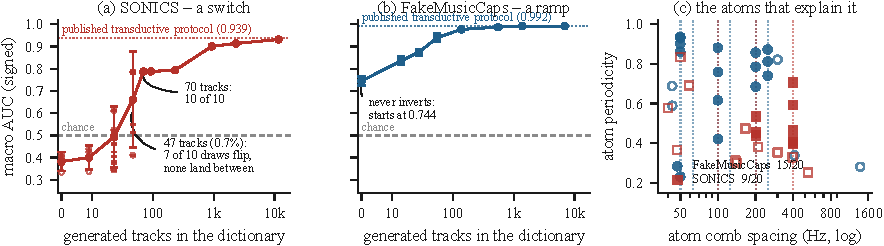
\includegraphics[width=\textwidth]{fig1_contamination.pdf}
\caption{\textbf{(a,b)} Unlabelled generated audio in the dictionary against detection
performance, held out, full corpus; circles are the three draws spanning the range and
ticks the four transition doses re-run at ten (\S\ref{ssec:dose}). \textbf{(c)} All
$K{=}20$ atoms per corpus, recovered comb spacing against periodicity; dotted rules
mark the \emph{measured} decoder spacings and their half and quarter, filled markers
lying within $1\%$ of one (\S\ref{sec:resolution}).}
\label{fig:contamination}
\end{figure*}

\section{Method and evaluation protocol}
\label{sec:method}

\subsection{The score}
We reimplement \cite{afchar2026finding} up to one documented difference. Each
track is reduced to the \emph{fakeprint} of \cite{afchar2025fourier}: a $16384$-point short-time Fourier
transform (STFT), a time average of the log power spectrum, subtraction of a
lower spectral hull and a clip at zero, leaving one non-negative peak height per
frequency bin in an analysis band. Stacking $n$ of them gives
$X \in \mathbb{R}^{n \times F}_{+}$, factorised as $X \approx HW$ with $K = 20$
atoms by multiplicative-update non-negative matrix factorisation (NMF; Frobenius
loss, NNDSVDA initialisation, $600$ iterations); a held-out track's $H_i$ comes
from the same solver run against the fixed $W$. Their formulation adds an
elastic-net penalty on $H$ and $W$ whose weights are not published, and we use the
unregularised factorisation; that penalty exists so an atom is learned ``only if a
sufficient collection of fakeprints follow a given pattern'' \cite{afchar2026finding},
which can only raise the count a generator needs to earn one, so \S\ref{ssec:dose}'s
dose is a lower bound on theirs. With $G$ a Gaussian blur along frequency, the score
of track $i$ is
\begin{equation}
  r_i = \lVert H_i W - H_i (W * G) \rVert_2 ,
  \label{eq:score}
\end{equation}
the peak energy the dictionary assigns to that track; the threshold is the quantile
$q$ of $r$ on real music alone. Note $r_i$ is unnormalised and inherits the scale of $H_i$. We use
$F = 7167$ bins and $\sigma = 2$ on FakeMusicCaps and $F = 4779$, $\sigma = 5$ on
SONICS (each corpus's full resolution, $\sigma$ scaling with bin width), chosen
once on the transductive protocol and fixed everywhere. Throughout,
signed macro AUC is the unweighted mean over the five generator families
of that family's AUC against all real music, oriented \emph{a priori} by the
mechanism (more comb $\Rightarrow$ more generated) and never flipped post hoc.

\subsection{The protocol axis}
Everything in \S\ref{sec:boundary} varies one thing, \emph{which unlabelled audio
forms $X$}: the scored corpus, a different corpus, real music only, or a simulated
catalogue with a known generated fraction. Labels \emph{construct} these fit sets
and are never seen by the estimator; (\ref{eq:score}) is identical in all four.

Both corpora are channel-matched first: every track, real or generated, is
% src: build_canonical_corpus.py --target-sr; canonical files read back at
%      16000 Hz (FMC) and 24000 Hz (SONICS), both classes, ledger R10.
%      CORRECTED: this sentence previously read "resampled to 16 kHz" for both,
%      which contradicted F=4779 below -- that dimension is only reachable at
%      24 kHz. The matching is WITHIN a corpus, which is what the argument needs.
% src: audio_preprocessing.CANONICAL_TARGET_LUFS = -23.0 (EBU R128); chain_kbps
%      64 on canonical_sonics_chain, 0 on canonical_fmc_raw16 (ledger F3).
%      CORRECTED 2026-09-22: this sentence read "-14 LUFS", which is the streaming
%      target, not the one the pipeline uses; and it omitted the MP3 stage entirely.
decoded, resampled to one rate per corpus ($16$\,kHz on FakeMusicCaps, $24$\,kHz
on SONICS), loudness-normalised to $-23$\,LUFS (loudness units relative to full
scale) and capped at a common duration ($9$\,s and $120$\,s), matched over the full
corpus rather than a split. SONICS additionally passes a shared $64$\,kb/s MP3
stage, the fake class's own format and the origin of that corpus's $7.35$\,kHz band
edge; FakeMusicCaps needs none. \S\ref{sec:confounds} shows why this is not
optional. SONICS supplies three Suno \texttt{chirp} and two Udio families against
$6{,}361$ reals;
FakeMusicCaps supplies MusicGen, AudioLDM2, MusicLDM, Mustango and Stable Audio Open
against $5{,}355$.

\subsection{Held-out dictionary evaluation}
\label{ssec:holdout}
A track in the fit set is reconstructed through atoms it helped create, so its
$r_i$ is inflated; if the fit reals are also the scored reals, the AUC inverts for
reasons unrelated to generated audio. On
% src: nmf_fmc_fitreals/ (leaked) vs nmf_fmc_curve_FINAL/ 0% cell (held out)
FakeMusicCaps the same quantity reads $0.167$ when the $600$ fit reals are
$100\%$ of the scored reals and $0.744 \pm 0.020$ over the full corpus with
dictionary rows excluded, a sign change produced entirely by the protocol.
All deployer-side numbers here are held out; the omission is invisible in the score
distribution, which is what makes it dangerous.

% =============================================================================
\section{The transductive dose}
\label{sec:boundary}

\begin{table}[t]
\centering
\caption{The published protocol against what a deployer can do. Full corpus,
$K{=}20$, full resolution; deployer rows are held out over three dictionary draws.
The proposed detector learns no dictionary, and is the only arm here correctly
oriented on all ten generator families.}
\label{tab:boundary}
{\footnotesize
\begin{tabular}{@{}lcc@{}}
\toprule
arm & \multicolumn{2}{c}{signed macro AUC $\uparrow$} \\
\cmidrule(l){2-3}
 & FakeMusicCaps & SONICS \\
\midrule
% src: nmf_{fmc,sonics}_FULL/nmf_peak_auc_lvl.csv | gates C1,C2 FAIL; C8 n/a
NMF on the scored corpus (published) & \textbf{0.9917} & \textbf{0.9389} \\
% src: nmf_fmc_fitsonics_FULL/, nmf_sonics_fitfmc_FULL/nmf_peak_auc_lvl.csv
NMF on a different corpus (inductive) & 0.5733 & 0.7123 \\
% src: nmf_{fmc,sonics}_curve_FINAL/nmf_peak_auc_lvl.csv, 0% cell, 3 seeds
NMF on real music only, held out & $0.744$ & $0.382$ \\
\midrule
% src: comb_{fmc,sonics}_HNULL/analytic_null_auc.csv | gates ledger R27.42, R27.45
proposed detector, no dictionary & \textbf{0.9445} & \textbf{0.8286} \\
\bottomrule
\end{tabular}}
\end{table}

\subsection{The boundary}
\label{ssec:boundary}
Table~\ref{tab:boundary} varies only the fit set. First, \emph{inductive transfer
is not no transfer}: a dictionary learned on the other benchmark still carries
signal, decoder combs being architecture-determined \cite{pons2021upsampling}. Second, the sign of the collapse is corpus-dependent.
FakeMusicCaps degrades to a usable $0.744$, which is what a deployer obtains,
whereas SONICS \emph{inverts}, real music scoring above generated. One ordering
remains unexplained: on FakeMusicCaps the
inductive dictionary ($0.5733$) is \emph{worse} than the reals-only one, so
contamination appears to need a generator match
% src: dict_{sparse,kmeans}_{fmc,sonics}_{pooled,reals}/nmf_peak_auc_lvl.csv --
% l1 sparse coding and k-means atoms reproduce the collapse on both corpora.
% Released rather than quoted: those cells predate \S\ref{ssec:holdout}'s correction,
% and the sentence was cut for space, not withdrawn.
(\S\ref{sec:conc}).

\subsection{The dose}
\label{ssec:dose}
Fig.~\ref{fig:contamination}(a,b) fits on half the real catalogue plus a known
number of unlabelled generated tracks, and scores the other half together with all
unused generated audio. On SONICS the mean curve rises smoothly between $23$ and $70$
contaminating tracks; the individual draws do not. Over ten draws per cell the number
% src: nmf_sonics_knee_10seed/nmf_peak_auc_lvl.csv, seeds 42--51, bins4779
with the correct sign is $0$ of $10$ at $23$ contaminating tracks, $7$ of $10$ at
$47$ and $10$ of $10$ at $70$, and at $47$ the two groups are disjoint in both
measures: macro AUC reads $0.78$--$0.79$ among those that flipped against
$0.41$--$0.55$ among those that did not, and the true-positive rate at a $5\%$
false-positive rate $0.45$--$0.47$ against $0.009$--$0.012$. The smoothness of the
mean is an artefact of averaging two regimes, and the experiment establishes
bimodality at a fixed dose rather than a threshold in dose. That dose is
${\approx}0.7\%$ of the unlabelled set at $K{=}20$, some $50$ generated tracks in
$6{,}400$, and it quantifies the ``sufficiently large sample collection'' that
\cite{afchar2026finding} states qualitatively. One reading is an atom
% src: nmf_sonics_K{5,10,40}_knee/nmf_peak_auc_lvl.csv, 3 seeds, bins4779
budget, and consistently the flipping dose falls from $168$--$341$ tracks at $K{=}5$
to ${\approx}47$ at $K{=}20$, though we cannot separate it from initialisation. Below ${\approx}5\%$ contamination on FakeMusicCaps one generator swings $0.21$
% src: nmf_fmc_curve_FINAL/nmf_peak_auc_lvl.csv, per-generator spread over seeds
AUC across draws where above $5\%$ it is stable to $0.003$, so below that level a
deployer obtains an unpredictable detector rather than merely a worse one.

% =============================================================================
\section{Controls: confounds, sign and resolution}
\label{sec:confounds}

\noindent\textbf{The delivery chain is a detector.} On the uncontrolled SONICS
% src: channel_sonics_UNCONTROLLED/, channel_sonics_chain_120s/ (ledger F6)
corpus one high-frequency floor statistic reaches signed AUC $0.98$, correctly
oriented on all five families; chain matching takes it to $0.60$ and costs the comb
statistic $0.217$ on that corpus. Every value below is measured after that chain.

\noindent\textbf{Signed AUC.} Reporting $|$AUC$|$ per generator inflated the comb
% src: comb_sonics_fmin{200,500,1000}/comb_auc_*.csv (signed and abs columns)
statistic's own SONICS macro from $0.6203$ to $0.8468$, the Udio families being inverted
where the chirp families are not: $|$AUC$|$ measures class information, not detector
performance.

\noindent\textbf{Which families invert is a property of the detector.} Below the
% src: nmf_sonics_curve_FINAL/nmf_peak_auc_lvl.csv, mix0pct, seeds 42--44
dose the dictionary score inverts on the three chirp families ($0.27$--$0.35$) and
sits at chance on the two Udio ones ($0.46$, $0.52$). The comb statistic does the
\emph{opposite} on the same corpus: chirp $0.88$--$0.94$, Udio $0.19$ and
$0.18$. Two detectors reading the same artifact fail on disjoint families, so a
sign verified once cannot be reused: it must be re-checked per detector, which is
% src: nmf_sonics_reals_energy/ joined to comb_sonics_FULL_rs15k/ on track_id --
% pooled, the dictionary score's correlation with the comb flips to -0.08 while
% energy stays +0.20: a failed between-class ordering, not lost within-family
% sensitivity. Cut for space, not withdrawn.
\cite{zhou2026fragile}'s criterion applied one level up. Because some families
% src: fusion_fmc_twosided/, nmf_sonics_twosided/, fusion_sonics_FULL_rs15k_* (F1)
invert we also adopt \cite{zisman2026realstats}'s real-only two-sided deviation
$|x - \mathrm{med}|/\mathrm{IQR}$, for median $\mathrm{med}$ and interquartile range
IQR, which over four arm-by-corpus cells costs $0.005$--$0.018$ where no family
inverts and gains $0.022$--$0.068$ where one does.

\noindent\textbf{Confound gates.} Every reported number carries an eleven-gate
battery, released with the code: channel, level, duration, silence, label
shuffle, score sanity, stratum survival, decoder-spacing concentration,
harmonicity, a content-identical control, and a bootstrap confidence interval (CI)
with a DeLong test \cite{delong1988comparing}.
% src: gate_nmf_FULL_c10/, gate_comb_fmc_c9/, gate_{nmf,comb}_sonics_FULL_120s/
Nine pass and two fail. Channel and level miss a criterion fixed in advance at $0.60$,
separating the classes at $0.61$--$0.63$ on both corpora: marginal failures,
precisely estimated at $n = 32{,}960$ but bounded, bandwidth-matched twins moving the
scores by only $-0.010$ and $-0.003$, so we bound the residual channel rather than
remove it. On the NMF arm decoder-spacing concentration
is \emph{not applicable}, a skip rather than one of the nine.

\noindent\textbf{Bandwidth is not the binding constraint; resolution is.}%
\label{sec:resolution}
The
comb's spacing is an architecture constant, not a data property
\cite{pons2021upsampling,odena2016deconvolution}, but its \emph{width} is set by
the analysis resolution, and both benchmarks are \emph{distributed} at $16$\,kHz, so
nothing survives above $8$\,kHz whatever container rate the chain of
\S\ref{sec:method} uses, which \cite{afchar2026finding} gives as a reason to work at
$44.1$\,kHz instead.
% src: nmf_{fmc,sonics}_FULL/nmf_peak_auc_lvl.csv, bins7167 / bins4779
With the band re-derived for the lower rate the method reaches
Table~\ref{tab:boundary}'s headline, so the cutoff is survivable and this family can
be evaluated on the corpora the field actually uses. Their published descriptor
transfers essentially unchanged: at its $4458$ dimensions, and at their physical
% src: nmf_{fmc,sonics}_binsweep/nmf_peak_auc_lvl.csv, bins4458/2600/1500/1000/445
resolution of ${\approx}2.7$\,Hz per bin, we measure within $0.010$ of the headline;
coarser resolutions bind, giving $0.9457$/$0.8368$ at $445$ bins. The requirement is a resolution, not a dimension, re-derived when the sample
rate changes.

\noindent\textbf{What the atoms are, and what the score fires on.} Counting an
% src: reports/figures/nmf_{fmc,sonics}_periodicity/atom_peakiness.csv
atom as \emph{on a comb} if its spacing lies within $1\%$ of a measured decoder
spacing or a sub-multiple, FakeMusicCaps places $15$ of $20$ atoms and SONICS $9$;
against the \emph{other} corpus's spacing FakeMusicCaps holds ($15$ against $7$,
Fisher $p = 0.025$) while SONICS cannot ($p = 0.18$), its spacing lying within
$0.12\%$ of twice FakeMusicCaps'.
% src: comb_{fmc,sonics}_HARM2/comb_per_track*.csv, modal candidate per family
The prior-restricted search attributes by a different route: at $M{=}2$ the
candidate it fires on concentrates per generator in
$85$--$99\%$ of tracks against $19\%$ for real music, at $49.8$\,Hz for MusicGen
\cite{copet2023musicgen}, $99.6$ for the three HiFi-GAN \cite{kong2020hifigan}
vocoders, $21.5$ for Stable Audio Open \cite{evans2024stableaudio}, and $49.8$ for
all three Suno families, whose $399.902$\,Hz comb is therefore its eighth harmonic.
Suno's decoder is proprietary and did not inform the candidate set: attribution on a
held-out architecture.

% =============================================================================
\section{A detector with no fit set}
\label{sec:detector}

% src: --average db --smooth-bins 5 --residual median --f-min 1000 (ledger R27.86)
\noindent\textbf{The statistic.} Each track is reduced to a time-averaged log power
spectrum from which a five-bin running median is subtracted, removing the spectral
envelope and leaving the narrow peaks; $e$ denotes that residual above $1$\,kHz. The
median replaces \S\ref{sec:method}'s clipped hull, which saturates teeth above
$5$\,dB where an autocorrelation peak needs their amplitude. Write $\mathcal{F}$ for
the discrete Fourier transform and $\tilde{e} = e - \bar{e}$ for the centred residual.
By the Wiener--Khinchin identity \cite{wiener1930harmonic} the autocorrelation
\emph{along frequency} is the inverse transform of the power spectrum,
$\rho_e(\tau) = r(\tau)/r(0)$ with $r = \mathcal{F}^{-1}\{|\mathcal{F}\tilde{e}|^{2}\}$,
evaluated on a zero-padded transform so that $r$ is linear rather than circular. A comb of spacing $\Delta$ is a peak of $\rho_e$ at lag
$\Delta/b$, for bin width $b$.

\noindent\textbf{The prior and the null.} The spacing is $f_s/\prod_l s_l$, and the
stride products of published decoders form a small enumerable set, so the search over
$\tau$ may be restricted to a prior $\mathcal{P}$: the lags at which a published
decoder could place a tooth. Restriction alone helps, but the restricted score still
inherits each track's residual statistics, and Udio's residual is \emph{flatter} than
real music's, which inverts it. We therefore score each track by
\begin{equation}
  m = \max_{\tau \in \mathcal{P}} \rho_e(\tau) - \max_{\tau \in \mathcal{N}} \rho_e(\tau),
  \label{eq:margin}
\end{equation}
% src: tests/test_null_alternatives.py fixture (ledger R27.38)
with $\mathcal{N}$ a null read on the same residual, so that the track's own
smoothness cancels. The choice of $\mathcal{N}$ is the detector. We take it to be
$\mathcal{P}$'s own hypothesis space, every lag an admissible fundamental could
reach, less a one-bin neighbourhood of \emph{every} integer multiple of \emph{every}
candidate. Excluding only $\mathcal{P}$ is insufficient: the comb's own higher teeth
then remain inside $\mathcal{N}$ and the score subtracts its own evidence, reading
$-0.128$ on a clean synthetic $50$\,Hz comb against $+0.511$ once the series is
protected. Because $\mathcal{N}$ is the alternative hypothesis and not an arbitrary
band, (\ref{eq:margin}) is a test rather than an offset, and the two sets are
disjoint by construction.

% src: hi_hz = 150 (R27.61); probe_M_{fmc,sonics}/ (R27.71, R27.76, R27.88);
%      comb_fmc_FULL/, fusion_sonics_FULL_rs15k_twosided/ (prior and null removed)
\noindent\textbf{Settings and ablation.} $\mathcal{P}$ holds the first $M$ multiples
of six published fundamentals spanning $21.5$--$100$\,Hz above a $40$\,Hz floor, and
$\mathcal{N} = \{\tau : 40 \le \tau b \le M{\times}150\} \setminus \bigcup_{\Delta,k}
\{\mathrm{round}(k\Delta/b) \pm 1\}$, the ceiling following from $150$\,Hz being the
highest plausible decoder fundamental. At $M{=}4$ this leaves $441$ admissible lags
on FakeMusicCaps and $253$ on SONICS; $M \in \{2,4\}$ moves macro AUC by at most
$0.007$ on either corpus, whereas $M{=}1$ costs $0.015$ and $0.029$, Stable Audio's
% src: probe floor 40 -> 20 Hz (ledger R27.62, R27.88)
$21.5$\,Hz series being unrepresentable above the floor. The floor itself is not
load-bearing: lowering it to $20$\,Hz, which admits that $21.5$\,Hz fundamental
directly, moves macro AUC by $-0.006$ and $+0.000$. Dropping the prior and the null
altogether reduces (\ref{eq:margin}) to the comb statistic of \S\ref{sec:confounds},
the maximum of $\rho_e$ over every lag, which reaches $0.9177$ on FakeMusicCaps and
$0.6864$/$0.7546$ (one-/two-sided) on SONICS but inverts on the two Udio families
(\S\ref{sec:confounds}): removing the dictionary removes the protocol dependence but
not the generator dependence, which the prior and the null remove.

% Decoy sets drawn at wrong frequencies, the
% construction we tried first, leave that collision to chance: they pin $19.5\%$ of
% FakeMusicCaps margins at exactly $0$, and a quantile threshold cannot be placed
% inside a tie mass, so recall at $q{=}0.95$ is $0.03$ on the worst family while the
% AUC reads $0.915$. The enumeration needs no seed and holds no tooth by construction.

% src: comb_{fmc,sonics}_HNULL/analytic_null_auc.csv | gates ledger R27.42, R27.45
The calibrated score reaches $0.9445$ $[0.9416, 0.9474]$ on FakeMusicCaps and
$0.8286$ macro on SONICS, whose pooled figure is $0.7925$ $[0.7887, 0.7963]$. Udio
reads $0.586$ and $0.579$, and no margin is tied at $0$.
Its gate profile is the comb statistic's own, and the
% src: c10_h4_{fmc,sonics}/recon_pairs.csv (ledger R27.46, R27.51)
% src: c10_sonics/, comb_recon_control/ (ledger K1) for the ablation's own pass
content-identical control passes on both corpora: within pairs from one source a
transposed-convolution codec \cite{defossez2023encodec} scores above its own source on
$93$--$98\%$ of pairs against $47$--$58\%$ for phase-only reconstruction, at chance on
FakeMusicCaps and barely detectable on SONICS at a median shift $33$--$40\times$ below
the codec's, so the score responds to deconvolution and not to re-synthesis. On Udio
it converts an inversion into a miss, a weaker outcome: three statistics agree Udio
leaves no comb in the analysed band.

\noindent\textbf{Prevalence and transfer.}%
\label{sec:deployment} At a $4.7\%$ false-positive rate the
% src: analysis_nmf_sonics_FULL/operating_points.csv, q=0.95, n_eval_reals=6361
dictionary score on SONICS recalls $67.4\%$ of generated tracks, a precision of
$0.127$ at a $1\%$ base rate. That ceiling belongs to the base rate, not the
detector, and is better stated as
% src: fpr_fma_h4/ precision-at-prevalence, inverted (ledger R27.89)
a requirement: precision $0.9$ needs a prevalence near $6\%$ at $q{=}0.999$ or $30\%$
at $q{=}0.95$. What differs between detectors is how a threshold \emph{travels}.
% src: fpr_fma_by_genre/, fpr_fma_h4/false_positive_rate.csv, q=0.95, n=2,998
On unseen Free Music Archive (FMA) \cite{defferrard2017fma} reals through an
identical chain the comb
statistic's false-positive rate moves from $0.042$ to $0.115$, $2.75\times$: a reals-only
quantile is a split-conformal threshold under exchangeability, and this violates
it. The proposed score instead lands under budget, $0.041 \to 0.030$
($0.72\times$, and again $0.72\times$ at $q{=}0.99$), while catching $87.6\%$ of
generated tracks.

\noindent\textbf{Per-genre error.} That error is not spread evenly. Across $2{,}998$
FMA tracks the comb statistic's false-positive rate is $0.236$ on Electronic ($n = 382$,
$95\%$ Wilson CI $[0.196, 0.281]$) and $0.028$ on Folk ($n = 359$), an $8.5\times$
spread with disjoint intervals; electronic production already carries quantised
% src: mondrian50_h4/, 50 calibration splits, alpha = 0.05 (ledger R27.34, R27.47)
spectral structure resembling a decoder comb.

% The proposed score can be equalised
% where the decoy calibration cannot, a quantile being unplaceable inside a tie mass:

Under group-conditional conformal calibration the proposed score holds all eight
genres between $4.4\%$ and $5.1\%$ against a $5\%$ target, a $1.17\times$ spread.
Frohmann et al.\ \cite{frohmann2025lyrics} note the same genres misfiring from
lyrics transcripts without quantifying a rate; in \emph{speech}, per-group
thresholds cut such disparity by $54$--$75\%$ at no cost \cite{fursule2026gender}.

\noindent\textbf{Cost.} No trainable parameter and no training, at $378$
% src: measure_efficiency.py, idle box, comb_priormax4_hmargin (ledger R27.57)
audio-seconds per second on four CPU cores, within $3\%$ of the uncalibrated statistic,
against MusicDET's $8.13$\,M parameters \cite{han2026musicdet}. It degrades $+0.2$/$+0.9$
points of equal-error rate under AAC- and Opus-64k, which preserve a
stride-determined periodicity, against $+13.6$ under time-stretch, a phase vocoder
that leaves the spacing in place and blurs its teeth.

% =============================================================================
\section{Conclusion and limitations}
\label{sec:conc}

A label-free score is not yet a zero-shot detector: the distance is $0.25$--$0.56$
AUC, bought by ${\approx}0.7\%$ unlabelled generated audio at $K{=}20$ and, on SONICS,
crossed between draws that are bimodal rather than noisy. Three things should
accompany any label-free number: which unlabelled audio the estimator saw, whether
fitted rows were scored, and the signed per-generator AUC. A detector told where to
look pays none of it: $0.9445$ and $0.8286$ with no fit set, no seed and no trainable
parameter.

\noindent\textbf{Limitations.} Two benchmarks that carry nothing above $8$\,kHz,
channel labelled by construction, with the channel and level gates missing a
pre-registered $0.60$ by $0.01$--$0.03$ on both; M6 \cite{li2026m6} or Echoes
\cite{pascu2026echoes} would test the dose under stronger shortcut controls. Channel
matching equalises rate, level and duration but not encoding history, a candidate
explanation for the corpus-dependent sign. Draws are three across the range and ten
% src: analysis_h4_fmc/, analytic_null_auc.csv recall_at_q95 (ledger R27.93)
at the transition; $\sigma$, $F$ and the prior's depth were fixed once and never
re-tuned per corpus; and the calibration of \S\ref{sec:detector} was devised after the
one-sided score fell short on SONICS, so its gain \emph{there} is post-hoc, the
FakeMusicCaps gain resting on a corpus that never motivated it. Its recall at a fixed quantile is
uneven where its AUC is not: $0.70$ and $0.80$ on MusicGen and Stable Audio Open
% src: probe_M_{fmc,sonics}/ macro deltas by prior depth (ledger R27.71, R27.76, R27.88)
against $0.93$--$1.00$ elsewhere.
% src: data/processed/robustness_hmargin/robustness_auc_eer.csv (ledger R27.58, R27.95)
The prior is also a scope limit: it assumes a strided transposed-convolution
decoder, so a synthesiser without one leaves no comb to find, and pitch-shift, which
resamples and moves $\Delta$ off all six candidates, drives the score \emph{below}
chance ($0.4665$) rather than merely degrading it. A log-frequency axis
\cite{dugelay2026improved}, on which that shift is a translation, is the obvious
repair, untested here.

\noindent\textbf{Future work.} \cite{afchar2026finding} report Udio among their
best detected at $44.1$\,kHz, which with \S\ref{sec:detector} predicts its comb
lies above both benchmarks' $8$\,kHz limit; wideband audio would settle it. Beyond
that: a \emph{third}-corpus contamination test for whether the dose needs a
generator match. Two
directions follow from the prior. Its modal candidate already concentrates per
generator (\S\ref{sec:resolution}), so the same statistic could \emph{identify} a
decoder and not only flag one, and a search that discovers spacings rather than
enumerating them would reach architectures the prior omits. Since $f_s/\prod_l s_l$
is fixed by the stack, editing a decoder's latent should change how strongly the comb
is expressed but not where it sits, which is directly testable.%
\label{endofbody}

\bibliographystyle{IEEEbib}
\bibliography{refs}

\end{document}
